Here we are going to to summarize the conventions that are being followed in this work.
\subsection{Einstein summation}
In this work we are using Einstein summation notation, which is a compact notation for expressing the sum of products of vectors in a vector space. In this notation, summation is implied whenever two indices appear in a product term, one subscript and one superscript. For example, the sum
\begin{align}
    a_i b^i = \sum_{i=1}^n a_i b^i
\end{align}
is implied by the notation. The summation convention is used in this work for all repeated indices, unless otherwise stated.
The summation convention applies to all repeated indices throughout this work unless stated otherwise. To simplify the notation further, we adopt a convention from MOFDFT \cite{zhang_m-ofdft_2023}, where a bar over a tensor indicates that pairs of indices corresponding to orbital basis functions of the same density are flattened into a vector. For example:
\begin{align}
    \text{tr}(\Gamma L^{\gamma})&=\Gamma_{\mu\nu}L^{\mu\nu,\gamma} = \bar\Gamma\bar L^{\gamma}\\
    \Gamma_{\mu\nu}\tilde D^{\mu\nu,\gamma\delta}\Gamma_{\gamma\delta} &= \bar\Gamma\bar {\tilde  D}\bar\Gamma
\end{align}
Here we interpreted $\bar\Gamma$ and $\bar L^{\gamma}$ as a vector and $\bar{\tilde D}$ as a matrix.
\subsection{Integral Notation}\label{integral_notation}
We are using Bra-Ket Notation, which is commonly used in quantum mechanics. For two functions $\phi,\psi:\mathbb{R}^3\rightarrow \mathbb{C}$ we denote:
\begin{align}
    \langle \phi | \psi\rangle &:= \int \phi(\mathbf r)\psi^\dagger(\mathbf r) d\mathbf r
\end{align}
As we are mostly interested in the ground state, which can be described by purely real functions, we can omit the dagger in the notation.
We also note hartree integrals by round brackets, for example:
\begin{align}
    (\phi | \psi) &:= \int \int \frac{\phi(\mathbf r)\psi^\dagger(\mathbf r')}{|\mathbf{r}-\mathbf{r'}|} d\mathbf rd\mathbf {r'}
\end{align}
\subsection{Data visualization}\label{boxplots}
To visualize distributions boxplots can give a good overview over the underlying statistics without overcrowding the plotwith to many information. The following visual guide demonstates how the plots used in the work are ment to be interpreted.
\begin{figure}[H]
    \centering
    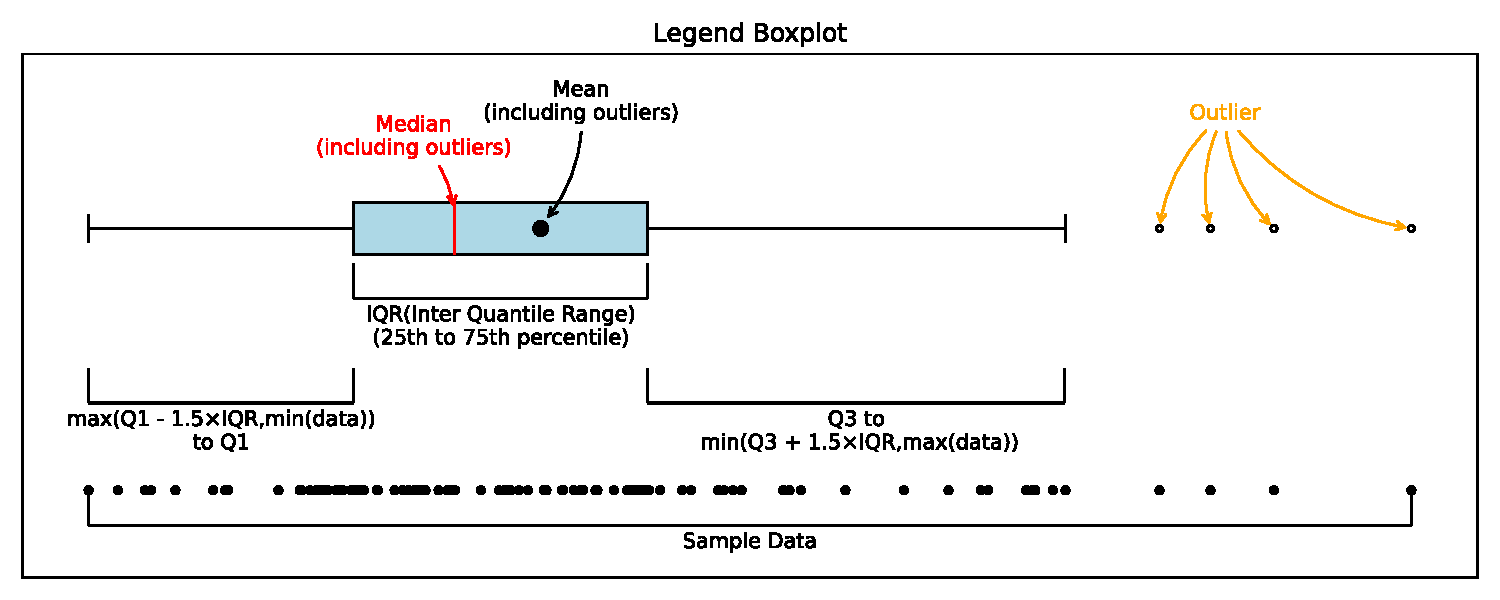
\includegraphics[width=1.\textwidth]{chapters/foundations/images_foundation/legend_boxplot}
    \caption{A boxplot showing the distribution of a toy data set with the important features labeled. Note that the left whiskers is shorted, which indicates that the data is right skewed.}
\end{figure}
Another challenge is the visualisation of the electron density of a molecule. In this work we are